\chapter{Introdu\c{c}\~{a}o} \label{chapter:intro}

A idade média da população mundial está aumentando progressivamente e, segundo estudos da~\ac{oms}~\cite{ageing2011}, muito em breve teremos mais idosos do que crianças. Ao considerar que a população idosa possui maior prevalência de doenças crônicas~\cite{prevcronica2009}, surge a necessidade de monitorar o estado da saúde dessa população. Portanto, diante do crescimento da quantidade de pacientes crônicos, da iminente redução do número de leitos hospitalares disponíveis e da insuficiência de profissionais especializados para atender esta demanda~\cite{healthmonitoring2013}, faz-se necessário transpor serviços de monitoramento dos pacientes crônicos dos leitos hospitalares para acompanhamento domiciliar~\cite{homecarebrazil2011}. 

Na averiguação desta demanda, a computação aplicada à saúde busca prover o monitoramento da saúde~\cite{healthmonitoring2013,bardram2010,aarhus_negotiating_2010}. Os ~\ac{sms} permitem ao médico acompanhar à distância o estado de saúde de seus pacientes colaborativamente~\cite{healthmonitoring2013}. Atualmente, os~\ac{sms} realizam tratamento preventivo e pró-ativo do estado de saúde~\cite{bardram2010}; suporte à reabilitação do paciente~\cite{sacbespoke2014}; e auxílio para o paciente atingir uma melhor qualidade de vida~\cite{sacsvmhms2014}. Referente ao monitoramento dos sinais motores, os~\ac{sms} quantificam estes sinais e conseguem quantificar as habilidades motoras~\cite{manumeterjbhi2014,patel_monitoring_2009}, efetuar análise da marcha \cite{robotgait2014} e identificar sinais de bradicinesia~\footnote{Sintoma do Parkinson que consiste na lentidão da execução dos movimentos.}~\cite{ambulatoryparkinson2010}. Contudo, o maior desafio dessas abordagens é motivar e induzir o usuário a executar movimentos específicos para o monitoramento da saúde motora.

Na busca por motivar os usuários, identificamos que os jogos eletrônicos encontram-se presentes na rotina diária de 26\% da população americana acima dos 50 anos~\cite{esa2016}. Com base nesse número, percebemos um público de jogadores idosos beneficiáveis por uma plataforma de monitoramento de dados de saúde embutida num jogo eletrônico. Aliado a esse estudo, foi encontrado, jogos voltados para o público idoso aplicados à melhoria do estado de saúde, tais como jogos para a persuasão da prática de atividades físicas~\cite{brox11} e jogos para a melhoria das capacidades físicas e cognitivas~\cite{arntzen2011}. 

É neste contexto de utilização, que os jogos eletrônicos foram utilizados para motivar o monitoramento da saúde, e induzir a execução dos movimentos específicos dentro do contexto de um jogo para a saúde. Mais especificamente, busca-se uma integrar os~\ac{sms} na vida diária de indivíduos através dos jogos, com foco em doenças motoras. Como objeto de estudo escolhemos \ac{dp} por ser uma doença neurodegenerativa crônica, progressiva e com causa desconhecida. É uma doença mais comum em idosos; no entanto, existem casos precoces em indivíduos antes dos 40 anos ou até mesmo abaixo dos 21~\cite{menezes2003}. A incidência da doença é estimada entre 100 a 200 casos por 100.000 habitantes e, com o envelhecimento da população, o contingente de pessoas diagnosticadas com~\ac{dp} tende a aumentar nos próximos anos. Após os 10 anos de tratamento, a doença leva o indivíduo a irreversíveis debilidades: motoras e cognitivas. Logo, a abordagem de monitorar os sinais em diferentes momentos do dia permite um melhor gerenciamento da doença e, por consequência, melhora a qualidade de vida destes indivíduos.


\section{Relevância}\label{section:relevancia}

Creating technologies for monitoring and creating body sensor networks has been the 
most active and successful research theme within pervasive healthcare – so far. One
strand of work is dedicated to achieving reliable monitoring of health signs like blood pressure, ECG, heart rate, skin conductivity, blood sugar, and similar. The main challenge has been to design and develop reliable yet non-intrusive, wearable sensors, which can be used by a layman. The goal has
been to create a platform for continuous monitoring, because substantial clinical evidence indicates that continuous monitoring of certain vital signs can work as early detector of different chronic diseases like hypertension, congestive heart failure, diabetes, dementia, and epilepsy. A related
strand is to make sure that this sensor and monitoring technology works together in a distributed infrastructure. This research relates to research within general sensor networks, and has been dedicated to the design and development of health-specific body sensor networks. Resilience, fail-over, network topology, wireless communication, protocols, and real-time data management are important issues in this strand of research~\cite{bardram2008}.

The OECD countries are facing a set of core challenges; an increasing elderly population; increasing number of chronic and lifestyle-related diseases; expanding scope of what medicine can do; and increasing lack of medical professionals. Pervasive healthcare asks how pervasive computing technology can be designed to meet these challenges. The objective of this paper is to discuss 'pervasive healthcare' as a research field and tries to establish how novel and distinct it is, compared to related work within biomedical engineering, medical informatics, and ubiquitous computing~\cite{bardram2008}.

J-BHI publishes original papers describing recent advances in the field of biomedical and health informatics where information and communication technologies intersect with health, healthcare, life sciences and biomedicine.  Papers must contain original content in theoretical analysis, methods, technical development, and/or novel clinical applications of information systems. Topics covered by J-BHI include but are not limited to: acquisition, transmission, storage, retrieval, management, processing and analysis of biomedical and health information; applications of information and communication technologies in the practice of healthcare, public health, patient monitoring, preventive care, early diagnosis of diseases,  discovery of new therapies, and patient specific treatment protocols leading to improved outcomes; and the integration of electronic medical and health records, methods of longitudinal data analysis, data mining and discovery tools. Manuscripts may deal with these applications and their integration, such as clinical information systems,  decision support systems, medical and biological imaging informatics,  wearable  systems, body area/sensor networks, informatics in biological and physiological systems,  personalized and pervasive health  technologies (u-, p-, m- and e-Health), telemedicine, home healthcare and wellness management. Topics related to integration include interoperability, protocol-based patient care, evidence-based medicine, and methods of secure patient data.~\cite{JBHI}


This paper describes computational approaches using evolutionary algorithms (EAs) that provide clinically relevant objective measures to identify and to quantify PD, both in humans and animal models. We begin by providing an overview of the diagnosis and monitoring of PD in humans. Thereafter two animal models of PD, the fruit fly (Drosophila melanogaster) and the zebrafish (Danio rerio), will be discussed. An overview of EAs will be provided and then a description of how we have used EAs
to study motor function in humans and animal models not only to provide effective classifiers for discrimination between disease and controls, but also between disease types.~\cite{compapproachparkinson2015}
The second important reason why PD patients require monitoring is for research studies. This typically involves serial detailed clinical measurements of impairment and disability using formal clinical rating scales. Whilst such scales allow a degree of standardisation across studies, they have a number of pertinent drawbacks such as length of time to complete the various assessments, limitations of using coarse-grained scales of severity, and the necessary subjective interpretation that results in inter-rater variability. Thus there is a real need for an accurate objective measure of PD clinical signs to improve the quality of monitoring for clinical and
research purposes~\cite{compapproachparkinson2015}
The subsequent analysis and classification of the data resulting from these sensors include conventional statistical approaches as well as machine learning including neural networks, support vector machine and EAs. EAs are the focus of the work presented in this paper and are considered in more detail in Section 4.~\cite{compapproachparkinson2015}








O surgimento de todas estas inovações tem convergido para viabilizar um paradigma de
computação proposto em 1991 por Mark Weiser [109] chamado de Computação Pervasiva.
Neste paradigma, não apenas dispositivos móveis têm capacidade de processamento e comunicação,
mas também vários outros objetos de uso diário, tais como: roupas, relógios, óculos,
dentre outros. A combinação do processamento e a troca de informações entre tais objetos
deve promover a adaptação do ambiente de acordo com as necessidades e desejos do usuário
sem que este, necessariamente, delibere sobre isso.
Diversos pesquisadores da área de computação pervasiva têm se preocupado com a área
de cuidados de saúde. A combinação destas duas áreas tem sido denominada de cuidado de
saúde pervasivo. Esta área tem sido apontada como uma área emergente de grandes impacto
e significância [103].
As pesquisas em cuidado de saúde pervasivo têm sido motivadas por estudos que apontam
que, ao tratarem de suas doenças em casa, pacientes passam a ter uma qualidade de vida
1
2
melhor do que se fossem acompanhados em hospitais [32; 110]. Além disso, alguns exames
geralmente sofrem alterações devido à ansiedade gerada nos pacientes quando estão em
ambientes clínicos. Desta forma, a acurácia no diagnóstico de um determinado quadro clínico
pode ser maior se a medição da mesma variável for feita no paciente ao longo do dia, em vez
de apenas uma única vez numa clínica [68].
Como posto por Bardram [11], cuidado de saúde pervasivo representa uma nova área
de pesquisa na academia e na indústria de computação. Uma evidência disto é a quantidade
de simpósios e conferências, apoiadas por entidades como SBC [98], ACM [1] e IEEE [49],
que vêm divulgando resultados de pesquisas na área, como são os casos do SBCUP [99],
UbiComp [106] e PerCom [91], respectivamente. Outros eventos também têm emergido com
o mesmo foco, ou relacionado, como são os casos do PervasiveHealth [92] e do FHIES [36].
No contexto de revistas científicas destacam-se as revistas IEEE Journal of Biomedical
and Health Informatics e Journal of the American Medical Informatics Association. Além
destas, outras revistas têm special issues na área, tais como: IEEE Transactions on Industrial
Informatics (special issue: Healthcare Systems and Technologies) e Sensors (special issue:
Cyber-Physical Systems).
Há na literatura trabalhos propondo que médicos, enfermeiros e outros profissionais de
saúde acompanhem pacientes à distância, mais especificamente em seus respectivos lares [40;
95; 104]. Outros propõem ferramentas de auxílio ao diagnóstico de situações de risco
eminentes ou mesmo de problemas respiratórios durante as fases de sono [18; 55; 83; 97;
112]. Uma característica comum presente nos trabalhos é o desenvolvimento de soluções
centradas no paciente, provocando uma maior participação deste no processo de tratamento
ou prevenção.
Por se tratar de um contexto crítico, ferramentas desenvolvidas para lidar diretamente
com a saúde de pessoas, principalmente aquelas sem supervisão humana, podem causar
danos irreversíveis aos pacientes, inclusive a morte. Assim sendo, tais ferramentas devem ser
consideradas sistemas críticos. Ou seja, é esperado que o desenvolvimento delas conte com
um suporte que forneça garantias de que a solução implementada se comportará conforme
especificado pelos profissionais de saúde. Esta garantia pode ser obtida por meio do uso de
técnicas formais de verificação de programas.
Diante do cenário exposto, é proposto no presente trabalho o uso de modelos formais na
1.1 Contexto de Cuidados de Saúde 3
concepção de sistemas para cuidado de saúde pervasivo. O domínio de aplicação abordado
neste trabalho é o auxílio à prática de exercícios físicos definidos por profissionais de saúde.
~\cite{elthon}


Dada a grande relevância do tema para a sociedade e seu impacto sobre os
custos de manutenção da saúde da população e qualidade de vida das pessoas,
diversas pesquisas têm sido desenvolvidas com o intuito de auxiliar o autogerenciamento
de pacientes. Mais especificamente, do ponto de vista de sistemas de
software, há soluções para suporte a diferentes etapas do tratamento, visando o
bem-estar do paciente durante a convivência com a doença. Tais pesquisas englobam
desde a utilização de mensagens instantâneas para notificar profissionais
quanto à resposta de pacientes crônicos à medicação prescrita [39], até a utilização
de sensores para monitoramento contínuo da movimentação do paciente [44] e do
seu estado de saúde [8] para antecipar possíveis situações críticas.
É nesse contexto de utilização de tecnologia de software para auxílio ao autogerenciamento
de portadores de doenças crônicas que se insere o presente trabalho.
Mais especificamente, propõe-se a utilização de sistemas de software para a
compatibilização entre os diversos planos de tratamento indicados por diferentes
profissionais de saúde, incluindo a gerência da evolução destes planos ao longo da
evolução da doença e do estado do paciente.~\cite{glauber}
Por fim, este trabalho foi o ponto de partida para a constituição de um grupo
de pesquisa na área de cuidados com a saúde e bem-estar, no Laboratório de Sistemas
Embarcados e Computação Pervasiva da Universidade Federal de Campina
Grande. Espera-se, portanto, que os desdobramentos deste trabalho sirvam de
base para futuros trabalhos de mestrado e doutorado na área.~\cite{glauber}



\section{Problemática}\label{section:problematica}
%Para a identificação do problema foi realizado uma Revisão Bibliográfica sobre os temas IEEE~\cite{ieee}, ACM~\cite{acm}, PubMed~\cite{pubmed}, Scielo~\cite{scielo}.

%A Revisão da Literatura objetivou encontrar problemas em aberto nos~\ac{sms}. Inicialmente Foi realizado, um estudo complementar nas diretrizes médicas para o suporte científico nesta área. Essa etapa teve como objetivo inicial identificar problemas nesses trabalhos que pudessem ser solucionados por esta tese.

Devido ao estilo de vida mais sedentário e ao aumento da população obesa, as pesquisas para a promoção da atividade física têm se tornado tópico de interesse para a comunidade científica~\cite{maitland2009,bartolome11,Mandryk2014}. Estudos demostram que uma atividade física regular traz benefícios físicos, cognitivos e emocionais~\cite{Mandryk2014}. Com o surgimento dos jogos comerciais, como o \textit{Wii Sports} da Nintendo~\footnote{http://www.nintendo.com}, em 2006, que aumentou a prática de atividade física de jogadores considerados sedentários~\cite{wiigraves2008}, é que pesquisadores da área de jogos para saúde buscaram apoiar essa prática com desenvolvimento de aplicações que motivassem a prática de atividade física~\cite{stacey2011}. Atualmente, os dispositivos de sensores de movimento permitem desenvolver jogos que promovem a saúde e o bem estar de forma promissora. Por esse motivo, houve um aumento significativo de jogos comerciais com o propósito de promover a saúde e o bem-estar da população~\cite{Papastergiou:2009:EPC:1570538.1570707}.


Os jogos pervasivos móveis motivam a atividade física de forma mais direta, tais como \textit{Transe}, \textit{Feeding Yoshi} e  \textit{Nokia Wellness Diary and Sports Tracker}, que promovem a saúde com a prática de atividade física~\cite{Suhonen:2008:SFE:1457199.1457204} e melhoram as condições de saúde por serem divertidos, imersivos e engajados. Para o público idoso, foram desenvolvidos diferentes jogos para a melhoria da saúde, como: sistemas para reabilitação motora dos idosos~\cite{brox11} e também para pacientes com~\ac{dp}~\cite{atkinson2010,synnott_wiipd_2012,sacbespoke2014}. 

Atkinson e Narasimhan~\cite{atkinson2010} desenvolveram um jogo que utiliza um sensor de toque para quantificar a habilidade motora do paciente com~\ac{dp}. Teoricamente, esta abordagem auxilia no diagnóstico do~\ac{dp}. No entanto, não foi realizado nenhum estudo com os pacientes para avaliar sua eficácia. Synnott \textit{et al.}~\cite{synnott_wiipd_2012} desenvolveu um sistema de gerenciamento medicamentoso e um jogo, utilizando um sensor de captura de movimentos, para identificar o sinal de tremor de~\ac{dp}. No entanto, o tremor de~\ac{dp} é de repouso~\cite{national2006parkinson}. Logo, quando o usuário está concentrado, entra no estado de ação e reduz drasticamente o tremor.

Papastergiou \textit{et al.}~\cite{Papastergiou:2009:EPC:1570538.1570707} identificaram efeitos positivos para a reabilitação através do uso do jogo \textit{Wii Sports} e um potencial mecanismo de prevenção e reeducação motora com o uso do \textit{Wii Fit}. Porém, esses jogos possuem suas limitações e não são substitutos dos esportes reais. Ainda assim, o autor salienta que um ambiente mais controlado, que permite a execução de atividades físicas, inibe a ocorrência de situações de risco como um movimento brusco e que venha causar um dano físico maior. Baseado nessas observações, esse trabalho primou por demonstrar as dificuldades e os efeitos positivos em combinar os jogos sérios de esportes e saúde com as tecnologias de sensores, para a personalização e adaptação dos jogos. Paraskevopoulos \textit{et al.}~\cite{sacbespoke2014} propõem um conjunto de diretrizes para o desenvolvimento de jogos com o objetivo de acompanhar o tratamento fisioterápico dos pacientes com~\ac{dp} e dar suporte à reabilitação 
destes.

Sinclair \textit{et al.}~\cite{Sinclair:2009:UVB:1515604.1515617} consideram que os jogos comerciais para prática de exercício físico (\textit{exergames}) não devem ser usados apenas como um motivador para a prática, mas também podem ser usados para monitorar sinais vitais como batimento cardíaco e reconhecer atividades via acelerômetros. Arntzen~\cite{arntzen2011} se preocupou com os aspectos cognitivos e físicos da aprendizagem baseada em jogos para idosos~\cite{arntzen2011}, defendendo que é necessário identificar quais habilidades cognitivas e físicas precisam ser desenvolvidas, além de considerar a limitação do idoso em relação aos movimentos bruscos no intuito de evitar lesões.

LeMoyne~\cite{lemoyne2010} quantificou os sinais de tremores de \ac{dp} usando \textit{smartphones}. Ele considerou que os \textit{smartphones} estão presentes na rotina dos pacientes e que estes iriam mensurar seus tremores em diferentes momentos do dia. No entanto, o principal problema em mensurar o tremor usando \textit{smartphones} é que o tremor do~\ac{dp} é de repouso~\cite{jankovic2008}. Logo, os pacientes reduzem drasticamente o sinal, o que impacta diretamente na coleta dos dados. Deve-se considerar também que LeMoyne~\cite{lemoyne2010} não realizou avaliações com pacientes ou estudo de caso-controle. 

% \begin{figure}
%  \centering
%  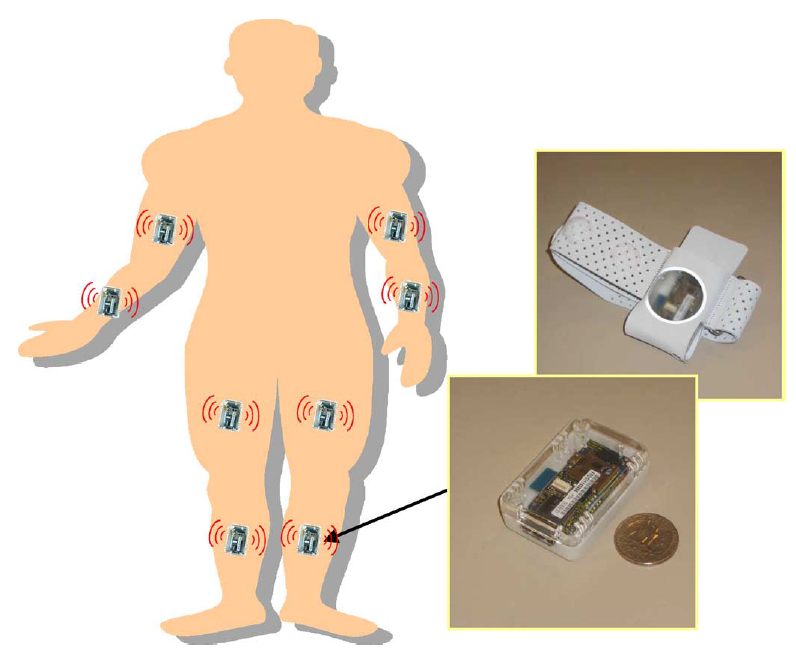
\includegraphics[scale=0.3]{./img/patel-shimmer.png}
%  % matrixargseg.png: 296x162 pixel, 100dpi, 7.52x4.11 cm, bb=0 0 213 117
%  %\caption{Estágio desenvolvimento de jogos ~\cite{fullerton2008game}}
% \caption[Disposição dos Sensores de Movimento (SHIMMER) no corpo no trabalho de Patel]{\textit{Disposição dos Sensores de Movimento (SHIMMER) no corpo no trabalho de Patel ~\cite{patel_monitoring_2009}}}
% %  \caption{Estágio desenvolvimento de jogos}
%  \label{fig:patel-shimmer}
% \end{figure}


% \begin{figure}
%  \centering
%  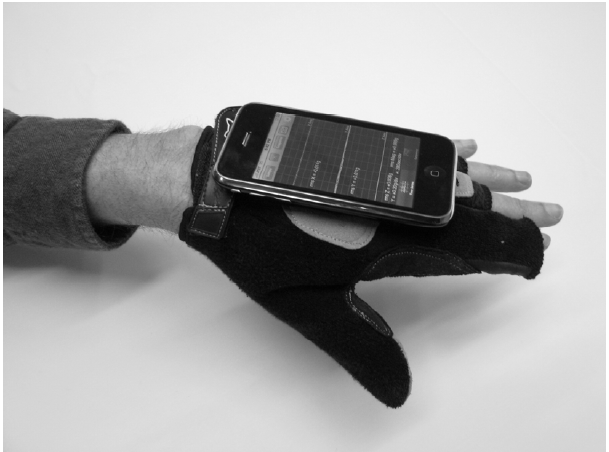
\includegraphics[scale=0.3]{./img/moyne-iphone.png}
%  % matrixargseg.png: 296x162 pixel, 100dpi, 7.52x4.11 cm, bb=0 0 213 117
%  %\caption{Estágio desenvolvimento de jogos ~\cite{fullerton2008game}}
% \caption[Aplicação para \textit{smartphone} com a finalidade de identificar sinais de tremor]{Aplicação para iPhone com a finalidade de identificar sinais de tremor ~\cite{lemoyne2010}}
% %  \caption{Estágio desenvolvimento de jogos}
%  \label{fig:iphone-tremor}
% \end{figure}

% \begin{figure}
%  \centering
%  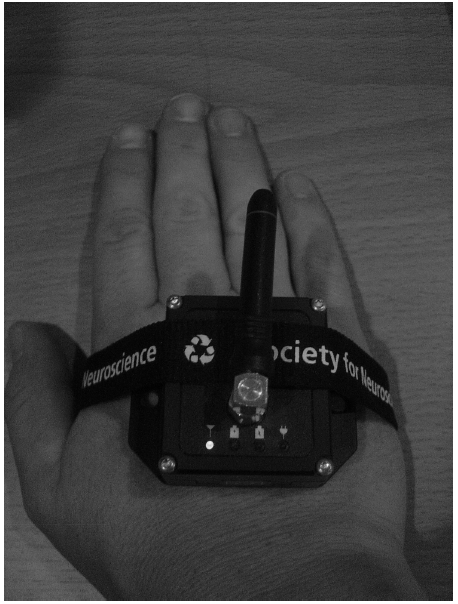
\includegraphics[scale=0.3]{./img/quantif-parkinson.png}
% \caption[\textit{G-Link Wireless Accelerometer} - Instrumento usado no trabalho de LeMoyne para quantificar o tremor da Doença de Parkinson.]{\textit{G-Link Wireless Accelerometer} - Instrumento usado no trabalho de LeMoyne~\cite{LeMoyne2009} para quantificar o tremor da Doença de Parkinson.} 
% %  \caption{Estágio desenvolvimento de jogos}
%  \label{fig:quantif-parkinson}
% \end{figure}

Em geral, as soluções existentes para \ac{sms} dos sinais motores utilizam sensores vestíveis (\textit{wearables}), que comumente são incorporados à roupa ou ao corpo do usuário. De acordo com a perspectiva do usuário, estes sensores são considerados invasivos e estereotipados~\cite{aarhus_negotiating_2010}. Por outro lado, o gerenciamento medicamentoso do~\ac{dp} necessita de um cuidado acurado e diário~\cite{quantitativeparkinson2011}. O problema então está em como alcançar o equilíbrio entre necessidade de monitoramento e não-invasividade e, ainda mais, buscando aumentar a motivação.

\section{Objetivos}
Neste trabalho, tem-se como objetivo a concepção de uma abordagem computacional não invasiva para o monitoramento de sinais motores. Jogos eletrônicos são utilizados como forma de motivar o monitoramento e abstrair o contexto de tratamento da saúde para os pacientes.

A Doença de \ac{dp} é utilizada como estudo de caso para a abordagem. Objetiva-se que o \ac{sms} integrado ao jogo eletrônico seja capaz de armazenar dados de sensores, processar sinais biomecânicos e identificar a presença do sinal de bradicinesia de \ac{dp}. Propõe-se uma arquitetura de software para SMS integrada a jogos eletrônicos e demonstra-se a viabilidade da mesma através da implementação de jogos com videogames disponíveis no mercado. 

A validação se baseia em duas etapas: na primeira, avalia-se a capacidade de monitoramento dos indivíduos com \ac{dp} em um estudo analítico de caso-controle; na segunda, avalia-se a possibilidade de inserir este monitoramento na rotina diária dos pacientes. O estudo analítico de caso-controle foi realizado com 30 sujeitos de pesquisa (15 do grupo controle e 15 diagnosticados com~\ac{dp}). Como resultado, identificamos e quantificamos o sintoma da bradicinesia. Para distinguir os grupos (caso-controle e diagnosticados com~\ac{dp}), utilizamos uma~\ac{svm} para classificação dos dados~\cite{datamining2005}, com a qual obtivemos uma acurácia de 86,66\%. Avaliamos a adequação da abordagem de monitoramento dos sinais motores na rotina diária usando jogos eletrônicos, aplicando a técnica~\ac{gqm}~\cite{van1999goal}. Como resultado, 90,00\% dos avaliados consideraram a abordagem não-invasiva e incorporável à rotina diária. 

\section{Metodologia}
Esta pesquisa foi submetida à avaliação pelo Comitê de Ética da UFCG (\textbf{CAAE: 14408213.9.1001.5182})~\footnote{Plataforma Brasil, url: http://aplicacao.saude.gov.br/plataformabrasil/} (Apêndice~\ref{sec:comite}), somente depois da aprovação deste é que os dados foram coletados. A metodologia de pesquisa possui aspectos qualitativos e quantitativos. Referente ao aspecto qualitativo, buscou-se identificar a importância desta tese junto à comunidade de especialistas da área de saúde (Seção~\ref{sec:entrevista_semi_estruturada}). Nos aspectos quantitativos, essa pesquisa fez uma análise do sensores de movimento e avaliou a acurácia da aquisição de sinais motores e possibilidade de identificar os sinais do~\ac{dp} baseado na Cinemática Angular do Movimento Humano. Por meio dos dados coletados, pudemos classificar a normalidade e dificuldade na execução de movimentos de abdução e adução dos braços~\cite{mcginnis2013biomechanics}, como será apresentado na Seção~\ref{sec:resultado_svm}. Para avaliar a aceitabilidade da proposta sob a perspectiva do usuário, utilizamos uma análise~\ac{gqm} a qual é uma abordagem hierárquica que inicia com objetivo principal e o divide em questões mensuráveis~\cite{saraiva2006}, como será apresentado na Seção~\ref{gqm_usuarios}.

Em resumo, três questões foram utilizadas como base para a definição da metodologia do trabalho em três diferentes etapas sequenciais:
	\begin{description}
	\item[ETAPA 1] Quais os benefícios de acompanhar os sinais motores do paciente diariamente, do ponto de vista do profissional da saúde?
	\item[ETAPA 2] Como melhor adquirir e quantificar sinais motores utilizando sensores de movimento para monitorar os sinais de \ac{dp}?
	\item[ETAPA 3] Na perspectiva dos usuários, a abordagem de quantificar os sinais motores é considerada não-invasiva e aplicável à rotina diária?
	\end{description}

As seguintes atividades foram realizadas para a execução do trabalho:

\begin{enumerate}

\item{Realizar revisão bibliográfica e coleta de requisitos junto a profissionais de saúde.}

\item{Definir o conceito da abordagem, denominada \ac{jogue-me}, baseada em captura de sinais motores através de sensores de movimento, utilizando jogos eletrônicos e processamento dos sinais para transformá-los em informações de saúde.}


\item{Analisar a perspectiva dos profissionais de saúde em relação ao acompanhamento dos sinais motores dos pacientes com~\ac{dp} (os profissionais foram indagados sobre a melhora na tomada de decisão quanto ao acompanhamento dos sinais) e verificar se os parâmetros motores, como velocidade angular e amplitude do movimento dos braços, são importantes para realizar o acompanhamento dos sinais do~\ac{dp}. Procurou-se encontrar, junto ao profissional de saúde, a importância do monitoramento dos sinais motores e os benefícios trazidos por este, através de uma abordagem de pesquisa qualitativa. Com esta pesquisa, foi possível validar a \textbf{ETAPA 1}, que consiste em verificar a importância do acompanhamento de sinais motores integrados à rotina diária do paciente.}

\item{Validar o uso de sensores para classificação dos dados através da classificação dos sinais motores adquiridos por sensores de movimento utilizados em jogos eletrônicos. A classificação consistiu em aplicar os sinais numa~\ac{svm} para distinguir indivíduos do grupo controle ante indivíduos diagnosticados com~\ac{dp}.
O resultado dessa pesquisa demonstrou a viabilidade da abordagem e, consequentemente, validou a \textbf{ETAPA 2} do trabalho.}

\item{Definir a arquitetura de software que viabilizou tecnicamente a abordagem~\ac{jogue-me}. Nesta etapa, definimos um arcabouço de software para encapsular o desenvolvimento de jogos com essa abordagem.}

\item{Validar a solução~\ac{jogue-me} do ponto de vista computacional. A solução foi validada através da implementação da arquitetura e do desenvolvimento de jogos. Com esta etapa, demonstrou-se ser possível realizar monitoramento de dados motores de forma não invasiva, ou seja, sem os jogadores perceberem que estão fornecendo dados de saúde.}

\item{Verificar junto ao público alvo (portadores de~\ac{dp}) os requisitos de usabilidade, adequação à rotina diária, segurança física e se a proposta é considerada invasiva na perspectiva do paciente. Com esta avaliação, validou-se a \textbf{ETAPA 3} da pesquisa.}

\end{enumerate}

\subsection{Termo de Consentimento Livre e Esclarecido (TCLE)}
Antes da realização da coleta dos dados, expomos aos sujeitos da pesquisa as informações necessárias para a realização do estudo. Desta maneira, o indivíduo consentiu com sua participação através da assinatura do Termo de Consentimento Livre e Esclarecido~\footnote{Resolução Nº 196/96, do Conselho Nacional de Saúde, do Ministério da Saúde (CNS/MS).} (Apêndice~\ref{sec:comite}). 

\subsection{Relação Risco Benefício da Pesquisa}
Os riscos inerentes podem decorrer da exposição de dados dos participantes da pesquisa, o que pode acarretar danos morais e/ou psicológicos. Por esse motivo, foram tomados todos os cuidados para que a identidade do indivíduo não fosse revelada, garantindo assim, privacidade e confidência das informações. Todos os dados coletados, estão disponibilizados para pesquisa futura, permitindo o uso para pesquisa a todas instituições envolvidas (UFCG, UFAL e IFAL). No entanto, preservamos a identidade dos participantes da pesquisa e omitimos todos os dados que permitissem sua identificação, conforme descrito no Termo de Consentimento Livre e Esclarecido.

Durante a realização da pesquisa com os participantes da pesquisa, houve uma preocupação referente a possíveis constrangimentos por parte do sujeito da pesquisa. Caso, não conseguisse realizar a pesquisa ou responder alguma pergunta devido ao comprometimento da doença. Os pesquisadores prestaram total assistência, orientando-os adequadamente. Mas, salientamos que os riscos apresentados justificam-se pelo benefício de monitorar os sinais do~\ac{dp} para um melhor tratamento da doença.


\subsection{Confidencialidade}
Os dados do estudo em questão são considerados propriedade conjunta das partes envolvidas (UFCG, UFAL e IFAL). Porém, sua utilização por terceiros necessita de prévia autorização de todos. No entanto, na submissão do Projeto ao Comitê de Ética da UFCG (\textbf{CAAE: 14408213.9.1001.5182}), expressamos o comprometimento em tornar público os resultados da pesquisa, sejam estes favoráveis ou não.


\section{Contribuições}
Atualmente, os jogos são aplicados para melhora da saúde em diferentes contextos. No entanto, nenhum dos trabalhos relacionados pretendem identificar sinais para monitorar o estado de saúde. Logo, este trabalho visa desenvolver um ambiente de jogo que motive a execução de movimentos específicos, com o propósito de quantificar os sinais motores dos usuários.

No entanto, alinhar a jogabilidade e a capacidade de monitoramento dos sinais de saúde não é trivial, pois deve ser levado em consideração o uso dos sensores e deve-se definir quais movimentos ou ações permitem a identificação dos sinais motores. Por este motivo, a proposta de um~\ac{sms} dos sinais motores usando jogos necessita de um acompanhamento de um profissional de saúde para supervisionar e auxiliar nas definições dos movimentos e ações dos usuários. 

%Posteriormente, na posse dessas ações, deverá ser testada a execução dessas atividades e sua aquisição para uma possível classificação dos dados conforme proposto nesta tese.
%os trabalhos já existentes~\cite{Ballegaard:2008:HEL:1357054.1357336,patel_monitoring_2009,visionbased2009,bachlin_parkinsons_2009,albanese2012}.
%De posse dos movimentos e da captura dos dados será feito um levantamento de um \textit{game design} que permita executar os movimentos em  um ambiente lúdico e divertido como um jogo para entretenimento ~\cite{sweetser2005-gameflow}.

Como possível cenário de uso para a pesquisa, supondo que um paciente de uma doença crônica como o~\ac{dp} faz uso de medicamento antiparkinsoniano e possui um jogo de monitoramento de sinais do~\ac{dp} em sua residência, caso ele utilize o jogo em diferentes momentos do dia, os sinais podem ser quantificados sem a presença de um profissional de saúde, que poderia visualizar a melhora ou piora do estado de saúde do seu paciente ao longo dos dias. A partir da presente abordagem, o médico, ao possuir a informação, poderia gerenciar melhor a dosagem medicamentosa e, consequentemente, prolongar a qualidade de vida do paciente~\cite{abn2010}.

\section{Organização do Documento}
O restante deste documento está organizado da seguinte forma:
\begin{itemize}
	\item No Capítulo~\ref{chapter:fundamentacao} está descrita a fundamentação teórica relacionada ao trabalho.
	\item No Capítulo~\ref{chapter:abordagem_gahme} está definida a abordagem \ac{jogue-me} de monitoramento de sinais motores não invasiva usando jogos eletrônicos.
	\item No Capítulo~\ref{chapter:arquitetura_captura} é demonstrada uma implementação da abordagem.
	\item No Capítulo~\ref{chap:avaliacao} são apresentados os experimentos realizados para validar a tese.
	\item No Capítulo~\ref{chapter:conclusoes_futuros} são apresentadas as conclusões do trabalho e propostos trabalhos futuros.
\end{itemize}
